\documentclass{article}
\usepackage{graphicx, verbatim, kotex} % Required for inserting images

\title{실습5}
\author{전형진 C011192}
\date{May 2024}
\begin{document}

\maketitle

\section{LISP 과제}

\subsection{LISP에 대하여}
LISP는 평소에 배운 명령형 언어와는 결이 다른 함수형 언어다. 우선 명령형 언어는 폰 노이만 컴퓨터 구조의 기반을 두고 효율성을 최대의 관심사로 두었다. 반면에 함수형 언어는 수학적 함수에 기반을 두고 있다. 견고한 수학적 함수이론에 기반을 두면서 오직 사용자의 친숙도를 높게 하는것이 주요한 관심사다. 그러다 보니 자연스럽게 프로그램이 돌아가는 컴퓨터 구조와는 거리가 멀어지게 되었다.

모든 자료를 연결 리스트로 처리하는게 특징이고, 함수이다 보니 괄호를 많이 쓴다. 명확한 표준화가 존재하지 않아 나중에 표준화된 common lisp가 등장하였다.

\section{a 코드의 설명 - NQueen}
nqueen은 backtracking 알고리즘의 대표 예제이다. backtracking은 상태 공간 트리를 그려 가능한 모든 솔루션을 탐색하는 알고리즘이다. 상태 공간 트리는 트리기 때문에 솔루션을 찾을 때는 DFS의 방식으로 탐색한다. 트리의 노드를 탐색할 때 이 노드가 가능한지에 대해서
boarding function을 이용해 탐색한다. 이 코드에서의 boarding function은 promising function이다. 함수 promising에서 서로 다른 두 퀸이 대각선에 있는지 열에 있는지를 판단한다. 함수 queens는 행 하나당 퀸 한개씩 열을 움직이며 배치한다. 재귀함수의 구조로 새로운 행과 열에 배치된 퀸은 기존의 퀸과 위치관계를 비교한다. 서로 잡아먹는 관계라면 함수 promising은 false를, 서로 잡아먹는 관계가 아니라면 함수 promising은 true를 반환한다. if문을 통해 promising이 true라면 다음의 행동을 한다. 퀸 n개를 모두 배치했다면 그때의 배치를 출력한다. 퀸이 남았다면 새로운 열에 퀸을 배치하고 맞는 배치인지 검사한다.

\newpage
\subsection{a 코드}
\begin{verbatim}
; 1. 조건에 부합하는 지 검사한다
; 2. 조건에 부합하고 i(현재 조사하고 있는 row 숫자) == n 같다면 출력한다.
; 3. 아니라면 다음 row에 j column에 퀸을 넣고 검사한다.
; 4. 재귀의 구조를 가지고 무한반복

(defvar n (read)) ; N을 입력받음
(setq a (1+ n)) 
(setq col (make-array a :initial-contents (make-list a :initial-element 0))) ; 퀸의 위치를 담는 배열인 col을 만듦.
; col[i] : i번째 row에 있는 퀸이 존재하고 있는 열의 값.

; Backtracking 알고리즘을 이용하여 코드를 구현함.
"
Backtracking에서 상태 공간 트리에서 추가적인 노드를 전개해도 되는지 유무를 판단하는 
Bording Function을 promising이라는 함수로 만든다. 이 알고리즘은 행을 기준으로 퀸이 자리할 위치를 판단한다.
"
(defun promising (a i) 
    (setq k 1) ; col[i]와 비교할 변수 col[k]의 k를 선언한다.
    (setq nswitch 1) ; 퀸을 놔도 되는지를 알려주는 nswtich 변수를 선언한다.
    "
    ; while문의 조건은 k가 i보다 작을 때 즉, 새로운 퀸을 둔(i, col[i])와 이전에 둔 퀸들의 좌표를 비교한다.
    
    "

"
밑의 조건은 두 퀸이 대각선에 있는지 판단한다. 
새로 놓은 퀸의 왼쪽 대각선 위쪽으로 전에 놓은 퀸이 있다면, col[i] - col[k] = i-k가 된다.
새로 놓은 퀸의 오른쪽 대각선 위쪽으로 전에 놓은 퀸이 있다면, col[k] - col[i] = k-i가 된다.
절댓값 함수인 abs를 이용하여 i-k가 나오면 대각선에 있는 것이기 때문에 loop를 종료하고 nswitch를 false로 둔다.
"
    
    (loop while (and (< k i) (equal nswitch 1)) 
        do (if (or (equal (aref a i) (aref a k)) ; col[i] == col[k]라면 두 퀸은 같은 열에 있는 것이다.  
            (equal (abs (- (aref a i) (aref a k))) (- i k)))         
            (setq nswitch 0)
        )
        (incf k) ; k값을 증가시키면서 값을 퀸들의 자리를 비교한다.
    )
    nswitch
)

(defun queens (a i) ; 알고리즘을 나타내는 함수이다.
    (if 
        (equal (promising a i) 1) ; 만약 promising 함수가 true라면 즉, 퀸들이 서로를 죽이지 않는 위치에 있다면 밑의 구문을 실행한다.
            (if (equal i n) ; 만약 퀸들을 모두 놓았다면 퀸들의 위치를 출력한다.
                (print a)
                (loop for j from 1 to n do ; 퀸을 모두 놓지 않았다면 다음의 구문을 실행한다.
                    (setf (aref a (1+ i)) j) ; 다음 열에 놓을 퀸을 정하고
                    (queens a (1+ i)) ; 새로운 알고리즘을 실행시켜 그 위치에 퀸이 있어도 되는지를 판단한다.
                )            
            )  
    )
)

(queens col 0) ; 알고리즘 시작  
\end{verbatim}
\newpage

\subsection{실행결과}
\begin{figure}[h]
    \centering
    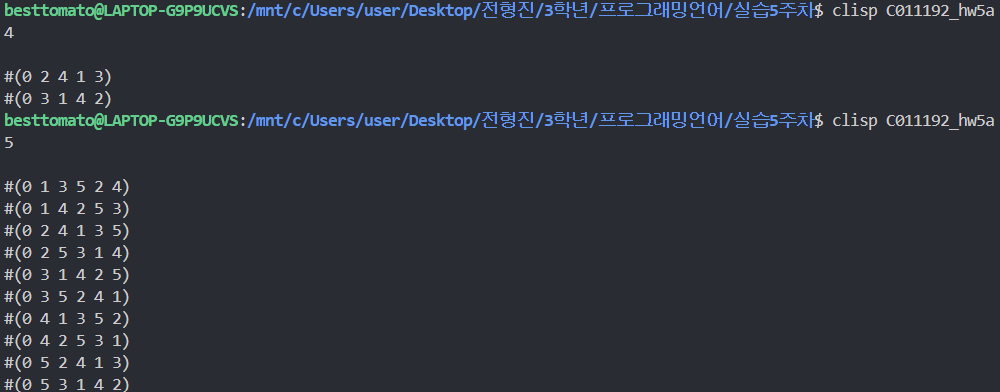
\includegraphics[scale = 0.7]{nqueenpic.png}
    \caption{nqueen 실행모습}
\end{figure}

\subsection{어려웠던 점}
1. 함수형 언어를 처음 사용하다보니 문법에 익숙하지 않았다.

처음 함수형 언어를 다뤘기 때문에 문법에 익숙해지는데 시간이 걸렸다. 함수형 언어 중 특히 lisp는 괄호를 굉장히 많이 쳐야 했기 때문에 이게 어떤 괄호인지 매번 헷갈렸다. 또한 리스트와 함수의 형태도 괄호의 형태로 되어 있기 때문에 겉모습이 헷갈렸다. 연산자가 괄호 맨 앞에 위치한 것도 코드를 작성하는데 애를 먹는 요소 중 하나였다.

2. nqueen 알고리즘에 익숙하지 않았다.

nqueen 알고리즘은 backtracking을 사용하면서 구현하는 알고리즘이다. 명령형 언어로 우선 nqueen 알고리즘이 어떤지 먼저 감을 잡았다. 그리고 알고리즘을 구현하는 데 꼭 필요한 boarding function과 재귀형태를 구현하려고 노력했다. 다만 명령형 언어보다 재귀를 구현하는데 있어서 함수형 언어가 조금 더 편했다. 아마 언어가 함수의 수학적인 논리를 그대로 따르고 있기 때문에 구현하기 쉬웠다는 생각이 든다.

\newpage
\section{b 코드의 설명 - InsertionSort}
삽입정렬은 배열을 정렬된 부분과 정렬되지 않은 부분으로 나누고, 정렬 안 된 부분의 가장 왼쪽 우너소를 정렬된 부분의 적절한 위치에 삽입하여 정렬되도록하는 정렬법이다. 정렬 안 된 부분의 숫자 하나가 정렬된 부분에 삽입됨으로써, 정렬된 부분의 원소 수가 1개 늘어나고, 동시에 정렬 안 된 부분의 원소 수는 1개 줄어든다. 
이를 반복해서 수행하면, 마지막엔 정렬이 안 된 부분엔 아무 원소도 남지 않고, 정렬된 부분에 모든 원소가 있게 된다. 단, 정렬은 배열의 첫 번째 원소만이 정렬된 부분에 있는 상태에서 정렬을 시작한다.
\subsection{b 코드}
\begin{verbatim}
(defvar n (read))
(print n)

"
입력받은 리스트의 원소들 중 첫번째 원소부터 자기가 들어갈 자리를 탐색한다. 코드에서
e가 바로 자기가 들어갈 자리를 직접 찾는 원소이다. e와 자기 바로 앞 인덱스의 원소와
크기를 비교하고 조건이 맞춰진다면 바로 앞 인덱스의 원소를 옮긴다.
"
(defun InsertionSort (a)
    (loop for next from 1 to (1- (length a)) ; list의 길이에서 1뺀 값을 가져온다.
        do  (setq e (nth next a)) ; for문에서 돌아가는 next의 인덱스를 가지는 리스트의 원소를 e라 한다.
            (setq i (1- next)) ; 인덱스 next-1 값을 i에 넣는다.                
        (loop while (and (>= i 0) (< e (nth i a))) ; i가 0보다 클 때, list a의 i번째 값이 e보다 큰지 비교한다.
            do (setf (nth (1+ i) a) (nth i a)) ; 만약 위의 조건을 만족하면 i+1번째와 i번째 원소를 스왑한다.
                (decf i) ; i를 늘린다
        )
        (setf (nth (1+ i) a) e) ; 빈공간이 생긴 i+1번째의 원소 자리에 e값을 넣는다.
        (print a) ; 매 과정을 출력한다.
    )
)

(InsertionSort n)
(print n)
\end{verbatim}

\newpage
\subsection{실행결과}

\begin{figure}[h]
    \centering
    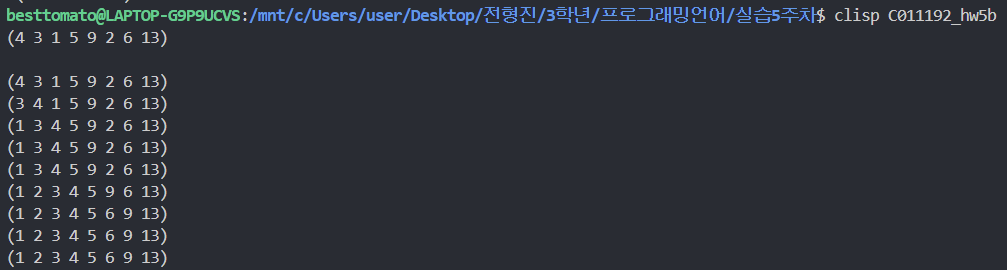
\includegraphics[scale = 0.7]{insortpic.png}
    \caption{InsertionSort 실행모습1}
\end{figure}

\begin{figure}[h]
    \centering
    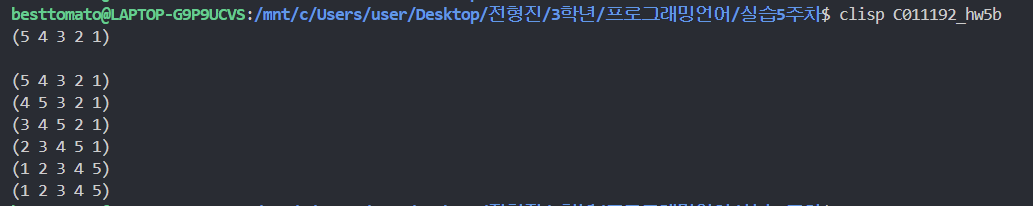
\includegraphics[scale = 0.7]{insortpic2.png}
    \caption{InsertionSort 실행모습2}
\end{figure}

\subsection{어려웠던 점}
마찬가지로 lisp의 문법이 익숙하지 않아 어려웠다. 그렇지만 nqueen 알고리즘보다 알고리즘 난이도는 낮아 만들기 수월했다.

\end{document}
